\section{Model}

Our starting model for the TMD system
is the effective tight-biding, low-energy, two-valley Bloch Hamiltonian
\cite{PhysRevLett.108.196802},
\begin{multline}
  H_τ^0 \ofK
  = a t \left( τ k_x σ_x + k_y σ_y \right) ⊗ I_2 \\
    + \frac{Δ}{2} σ_z ⊗ I_2 - λ τ \left(σ_z - 1 \right) ⊗ S_z.
\end{multline}
The operators $σ_i$ are Pauli operators acting
on the two Bloch orbital states
$\ketOrb{ν}{\ofK}$
(indexed by $ν = ±$ and which only involve the angular momentum $d$-orbitals
$\Ket{d_{x^2 - y^2}} + i τ \Ket{d_{xy}}$ and $\Ket{d_{z^2}}$)
such that $σ_z \ketOrb{±}{\ofK} = ± \ketOrb{±}{\ofK}$.
The valley index $τ = ±$, corresponding to the $± \vc{K}$ points,
and the spin index ${\s} = ±$ (or ${\s} =\ ↑↓$),
corresponding to the $z$-component of the spin through $s_z = {\s} / 2$,
are good quantum numbers.
The momentum $\vK$ is measured from the valley center,
i.e., for a given valley, the total momentum relative to the center
of the Brillouin zone is $\vK + τ \vc{K}$.
The energy gap is $Δ$, the spin splitting in the valance band is $2 λ$,
the lattice constant is $a$, and $t$ is the effective hopping integral.

The energy spectrum,
\begin{equation}
  \label{eq:energy}
  \fnEnergy{n} \of{k}
  = \frac{1}{2} \left( λ τ {\s} + n \sqrt{{\left( 2 a t k \right)}^2
  + {\left( Δ - λ τ {\s} \right)}^2} \right),
\end{equation}
with $n = 1$ ($n = -1$) indexing the conduction (valence) band
is shown in \cref{fig:energy}.
\begin{figure}
  \caption{%
    Energy bands for $\ce{WSe2}$ as given by \cref{eq:energy}
    with $a t = \SI{3.939}{\electronvolt \per \angstrom}$,
    $Δ = \SI{1.60}{\electronvolt}$,
    and $λ = \SI{0.23}{\angstrom}$.
    Each valley is centered at $± \vc{K}$ relative to the center of the
    Brillouin zone.
    The energy for a given band depends only on the distance $k$
    measured from the valley center.
  }\label{fig:energy}
  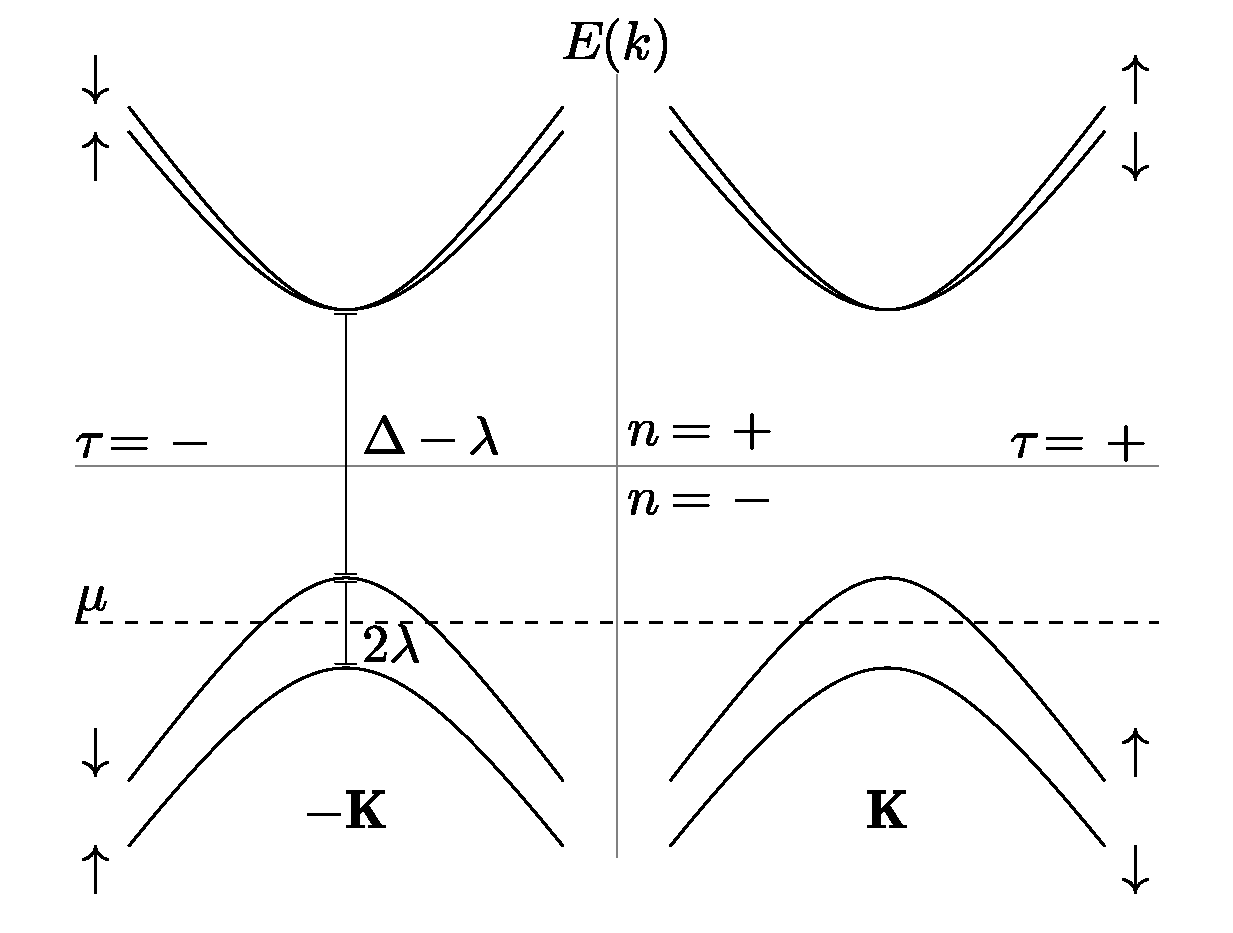
\includegraphics[width=\columnwidth]{figures/energy-bands}
\end{figure}
We focus on systems which have been doped
such that the chemical potential $μ$ lies in the upper valance bands.
Within each band, the Bloch basis eigenstates are written
in terms of the orbital states as elements on the Block sphere,
\begin{equation}
  \begin{aligned}
    \Ket{u_{τ {\s}}^n \of{k, ϕ}}
    = & \cos{\frac{\fnTheta{n}}{2}} \ketOrb{+}{\of{k, ϕ}} \\
    + e^{-i τ ϕ}
      & \sin{\frac{\fnTheta{n}}{2}} \ketOrb{-}{\of{k, ϕ}},
  \end{aligned}
\end{equation}
where $k_x + i τ k_y = k e^{i τ ϕ}$ and
\begin{equation}
  \tan{\frac{\fnTheta{n}}{2}}
  = \frac{a t τ k}{\dfrac{Δ}{2} - \fnEnergy{-n} \of{k}}
  = \frac{a t τ k}{\fnEnergy{n} \of{k} - \fnEnergy{-} \of{0}}.
\end{equation}
Note that the polar angle on the Bloch sphere
of the conduction and valence bands are related by
$\fnTheta{-} - \fnTheta{+} = τ π$.
The mapping of the energy band to the Bloch sphere,
parametrized by $\left( θ, ϕ \right)$,
encodes the topological character:
as one moves from the node out to infinity,
the states sweep either the northern or southern hemisphere
with a chirality determined by the Berry curvature.
